\subsection{Keypoint-Based Visual SLAM}
\label{sec:kv_slam_background}

SLAM is the joint problem of simultaneously generating a map of an environment and estimating the position of an observer within that map based on sensor observations. First explored in the 1980s \cite{smithEstimatingUncertainSpatial1988}, SLAM has become a de facto standard in robotics for tasks which require operations within unfamiliar environments. A wide variety of sensors can be utilized by SLAM, the most common being LiDAR, cameras, and RGBD sensors. The high level relationships between these sensor modalities are shown in Figure \ref{fig:slam_family_tree}. Keypoint-Based Visual SLAM refers to a subset of the wider SLAM ecosystem characterized by the use of cameras as the primary sensor, and image features extracted from images as the primary data for tracking and mapping.

\begin{figure}[!ht]
    \centering
    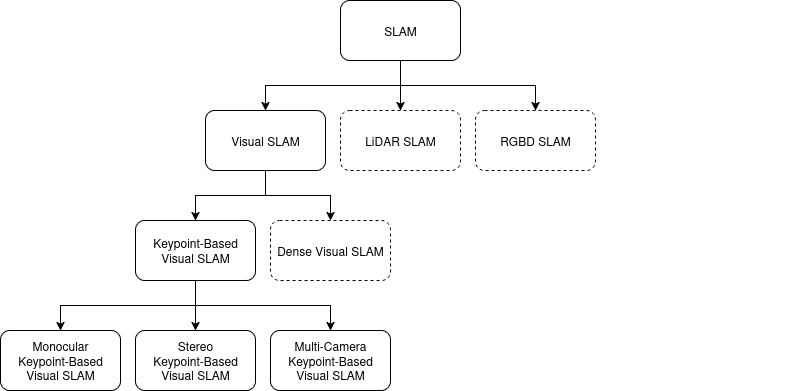
\includegraphics[width=0.9\textwidth]{resources/slam_family_tree.png}
    \caption[SLAM Family Tree]{Overview of the relationships between popular SLAM modalities.}
    \label{fig:slam_family_tree}
\end{figure}

The first implementations of KV-SLAM came in the early 2000s \cite{seMobileRobotLocalization2002}\cite{davisonRealtimeSimultaneousLocalisation2003}, making the field relatively young. This can be attributed to the difficulty in estimating 3D geometries from 2D images, unlike LiDAR and RGBD which are capable of direct 3D environmental measurements. However, due to the extremely low cost and wide availability of camera sensors, KV-SLAM is a popular modality for robotics, AR/VR, and autonomous driving applications. A full description of the internal operations of KV-SLAM is out of scope for this thesis, but an overview of key concepts relevant to this research is given below, followed by a discussion of the KV-SLAM subsystems which are relevant to this research.

\subsubsection{Image Features}

An image feature is the combination of a keypoint and a feature descriptor \cite{loweObjectRecognitionLocal1999}. Keypoints are locations in an image which are (ideally) invariant to lighting, scale, translation, and rotation\cite{shiGoodFeaturesTrack1994}, while descriptors are a data vector that acts as the unique fingerprint for the feature. Keypoints are located, and their descriptors generated in a process called feature extraction.

The output of feature extraction is a set of image features, which when combined are significantly smaller than the image from which they were extracted. Figure \ref{fig:feature_extraction_and_matching} shows the output of the ORB feature extractor, along with how the features extracted between two images can be matched by their descriptors. The capability to match the same set of points across multiple viewpoints is core to how 3D map points are estimated from multiple 2D images.

\begin{figure}[!ht]
    \centering
    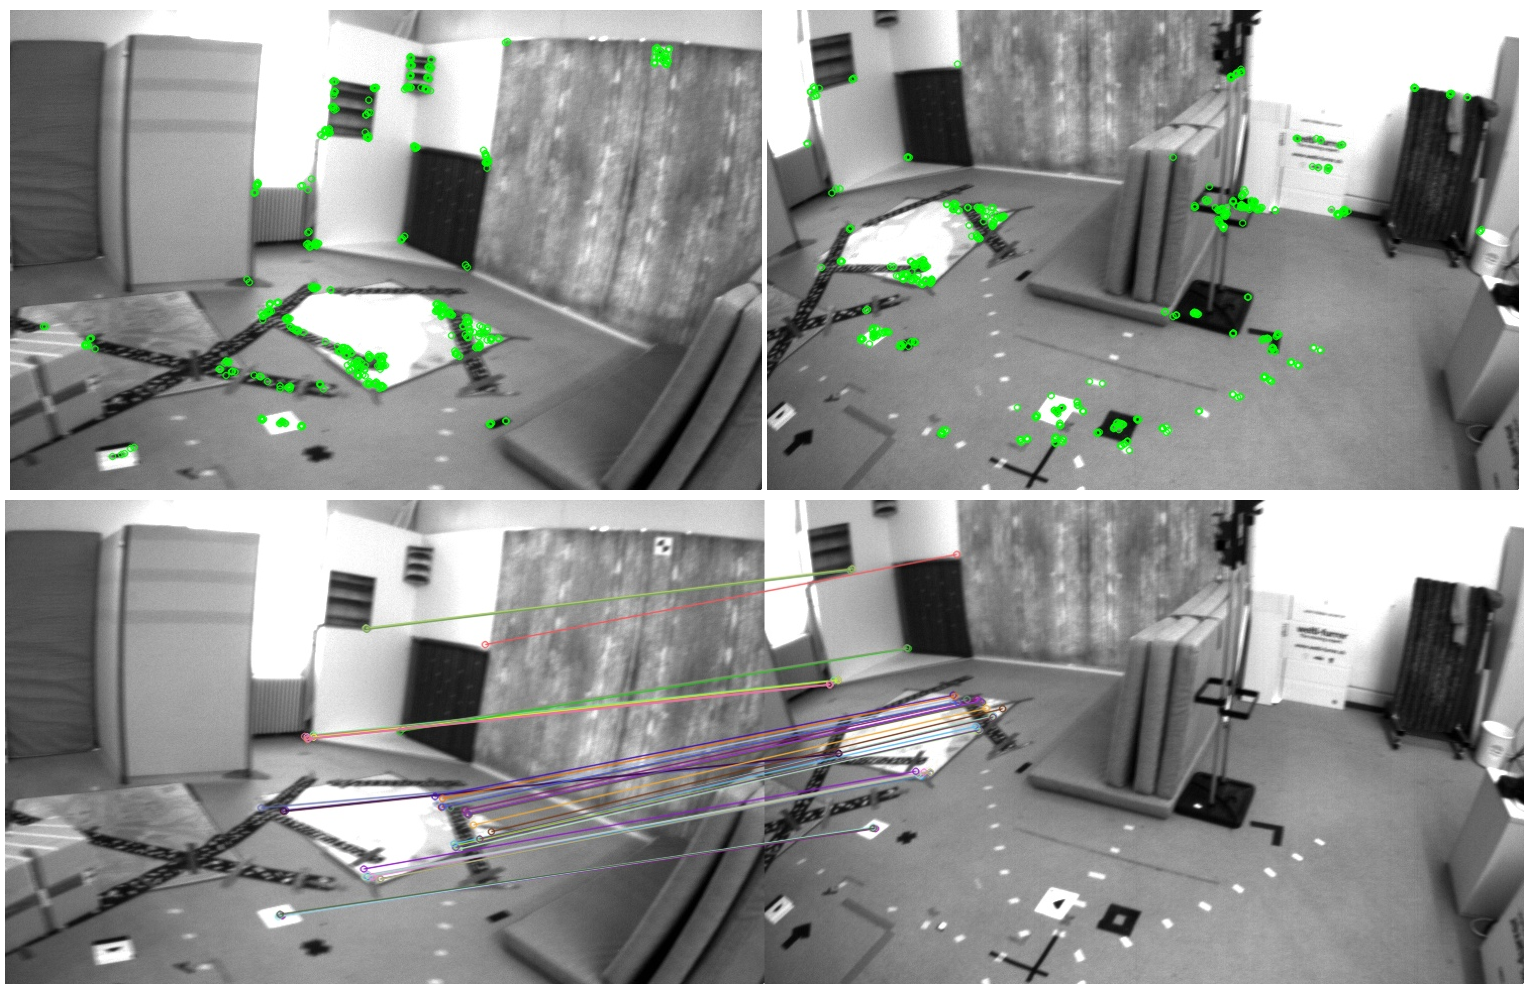
\includegraphics[width=0.9\textwidth]{resources/feature_extraction_and_matching.png}
    \caption[Image Feature Extraction and Matching]{(Top) ORB features extracted from two frames of the EuRoC MAV V1\_03 dataset \cite{burriEuRoCMicroAerial2016}. (Bottom) Corresponding ORB feature matches between the two frames.}
    \label{fig:feature_extraction_and_matching}
\end{figure}

It should be noted that map point matching is far from perfect. Feature descriptors tend to be based on the pixel values surrounding the keypoint location, meaning that visually similar image features will have similar descriptors. This is desirable and necessary to find feature matches between image frames, but means that in areas with repeating patterns or low visual texture, false matches are common.

\subsubsection{Random Sample Consensus (RANSAC)}

Through epipolar geometric methods, the relative transforms between two images which contain eight or more common and matched points can be uniquely\cite{longuet-higginsComputerAlgorithmReconstructing1981}\cite{hartleyDefenseEightpointAlgorithm1997}. But as shown above, the process of extracting and matching image features is noisy, and will contain outlier data, meaning that an incorrect solution or no solution may be found. The solution to this issue is the Random Sample Consensus algorithm.

The RANSAC algorithm is very easy to understand visually. Let's imagine a sensor measures linear data, but introduces some normally distributed noise about the true measurement. Additionally, the sensor has a bug which causes about 20 percent of the readings to be outliers. The output produced by such a sensor may look like the left most plot of Figure \ref{fig:ransac}. As can be seen, the best fit for all the data is far from correct due to the outliers. By iteratively selecting a random sample of the input data, fitting the model to this sample, and counting the number of inliers, RANSAC can find a solution which explains the highest proportion of the observations.

\begin{figure}[!ht]
    \centering
    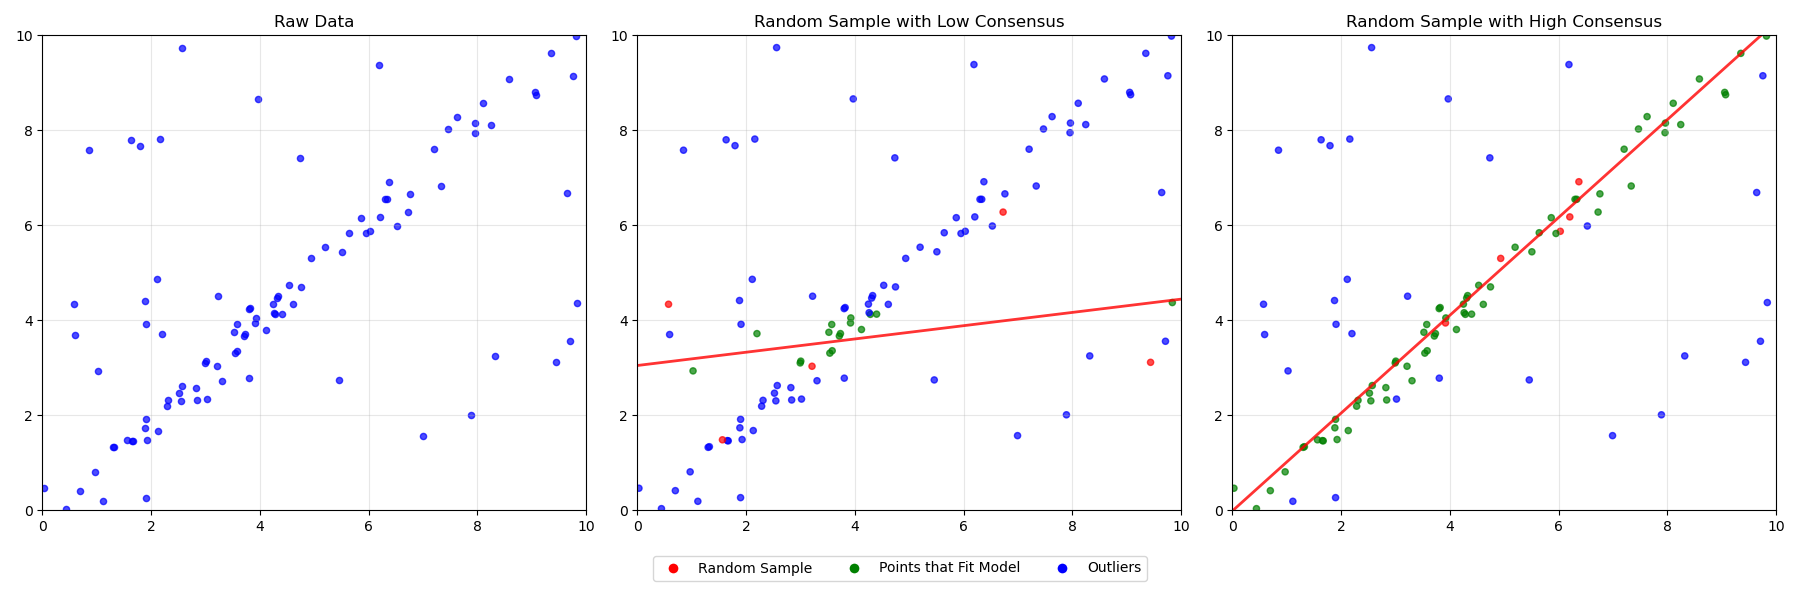
\includegraphics[width=0.9\textwidth]{resources/ransac.png}
    \caption[2D RANSAC Example]{A demonstration of how RANSAC determines model parameters through iterative random sampling and model application.}
    \label{fig:ransac}
\end{figure}

\subsubsection{KV-SLAM Subprocesses}

It is difficult to conceptualize modern SLAM as a pipeline from inputs to outputs. While implementations differ significantly, KV-SLAM can be better understood as a collection of tightly coupled concurrent processes. Figure \ref{fig:subprocesses} shows a block diagram of the layers and subprocesses of a modern KV-SLAM system. A complete understanding of each subprocess is not necessary, so we offer a high level overview here, with additional detail given to processes which can be improved through the implementation of the viewpoint-aware point removal method.

\begin{figure}[!ht]
    \centering
    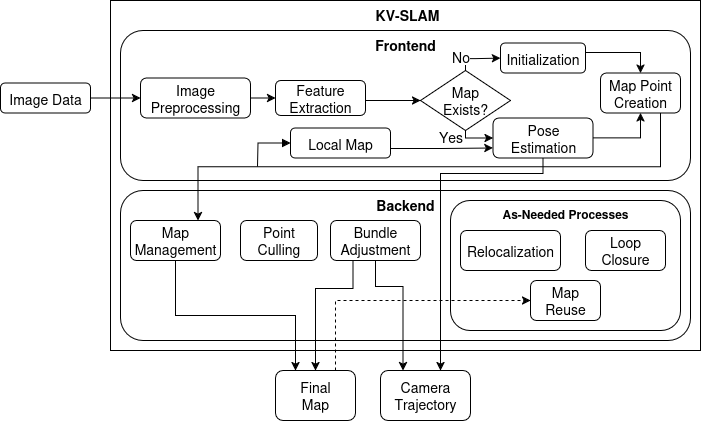
\includegraphics[width=0.9\textwidth]{resources/subprocesses.png}
    \caption[KV-SLAM Subprocesses]{The inputs, outputs, and subprocesses of a model simplified KV-SLAM system.}
    \label{fig:subprocesses}
\end{figure}

The frontend is responsible for coarse motion estimates and map point generation. It is capable of determining 3D relative motion between two images in the case of initialization, or localization within a small local map in the case of pose estimation. The frontend needs to be extremely fast, as running slower than the frame rate of the camera would lead to a backlog of images to process, and would prevent real-time performance. To that end, the frontend assumes small-scale, continuous motion between frames, and does not handle discontinuities well.

The backend is responsible for integrating the coarse motion estimates and map points from the frontend into the larger context of the global map and trajectory. There will always be some error in the motion and map point estimations from the frontend, so the backend adjusts various elements of the global estimate such as frame positions, map point positions, and camera parameters to minimize the overall error within the global estimation in an optimization process called bundle adjustment \cite{triggsBundleAdjustmentModern2000a}. The backend processes tend to run at a slower rate than the frontend, focusing on providing global consistency that the frontend cannot produce alone.

Within this model, the VD-OMR system being researched would reside in the backend, specifically under the point culling subprocess. The purpose of point culling is to reduce the overall size of the map by 